Сверточные нейронные сети (CNN)\cite{lecun1989handwritten} представляют собой класс глубоких нейронных сетей, специально разработанных для обработки структурированных данных, таких как изображения. Они эффективно работают за счет своей способности автоматически извлекать иерархические признаки из входных данных, что делает их особенно подходящими для задач компьютерного зрения.

Основными компонентами сверточных нейронных сетей являются сверточные слои, пулинг слои и полносвязанные слои. Сверточные слои выполняют операции свертки над входными данными с использованием фильтров или ядер, чтобы извлечь локальные пространственные признаки, такие как грани, углы и текстуры. Это позволяет модели обнаруживать абстрактные особенности изображений на разных уровнях детализации.

Пулинг слои предназначены для уменьшения пространственных размеров активаций, полученных после сверточных операций, путем объединения значений пикселей в заданных областях. Это позволяет модели быть инвариантной к небольшим трансляциям объектов на изображении и уменьшает количество параметров, что способствует предотвращению переобучения и повышению эффективности вычислений.

Полносвязанные слои обычно располагаются в конце архитектуры нейронной сети и используются для объединения высокоуровневых признаков, извлеченных предыдущими слоями, в предсказания или классификации. Эти слои обладают полным соединением со всеми активациями предыдущего слоя и представляют собой типичные слои нейронных сетей, в которых каждый нейрон связан с каждым нейроном предыдущего слоя.

Во время обучения сверточной нейронной сети параметры каждого слоя оптимизируются с использованием методов оптимизации, таких как обратное распространение ошибки и стохастический градиентный спуск, с целью минимизации заданной функции потерь. Этот процесс позволяет модели настраивать свои параметры для эффективного извлечения признаков и выполнения конкретной задачи, такой как классификация изображений или сегментация объектов.


\begin{figure}[h]
    \centering
    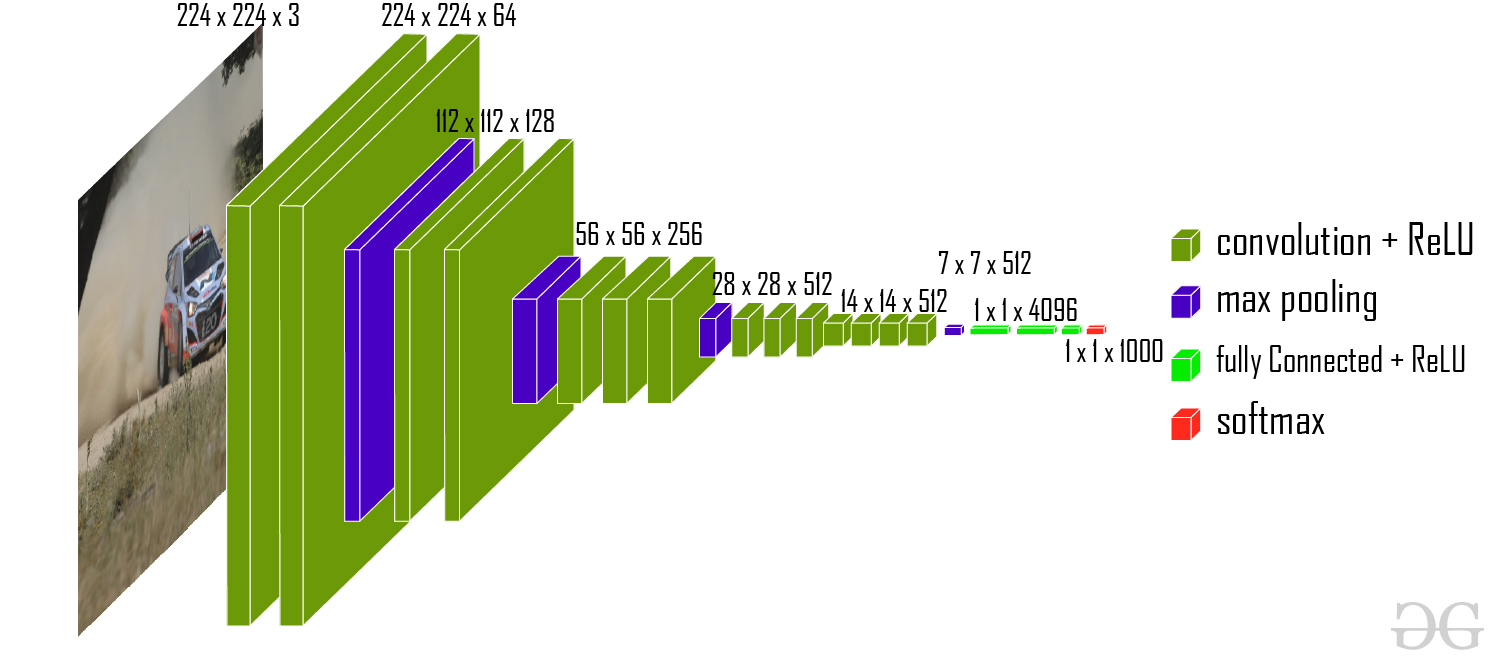
\includegraphics[width=0.5\textwidth]{assets/cv/vgg16.jpg}
    \caption{Архитектура VGG16 \cite{simonyan2014very}}
    \label{vgg_arch}
\end{figure}


Архитектуры U-Net \ref{unet_arch}  и ResNet \ref{vgg_arch} являются двумя широко используемыми моделями в области компьютерного зрения, обе из которых имеют уникальные характеристики и применяются в различных задачах.

U-Net - это архитектура, разработанная для сегментации изображений, особенно в медицинском изображении. Ее особенностью является использование симметричной структуры, включающей свертки (downsampling) для уменьшения размерности и деконволюционные слои (upsampling) для восстановления пространственного разрешения. Основное преимущество U-Net заключается в способности эффективно обрабатывать маленькие объекты и сохранять детали на всех уровнях.

\begin{figure}[h]
    \centering
    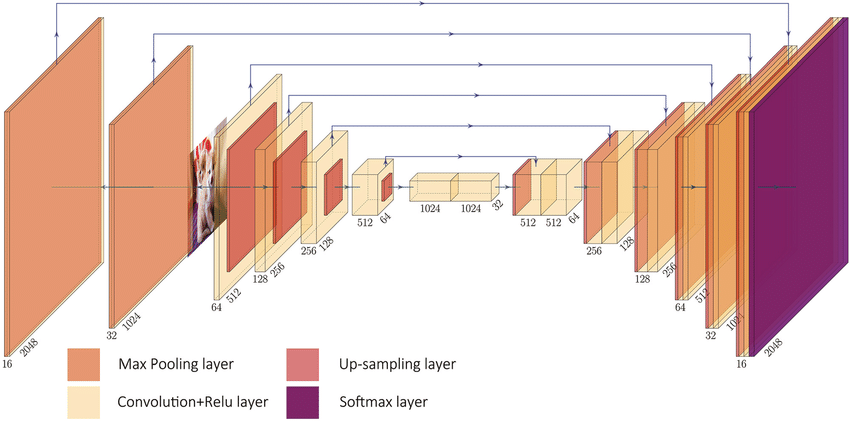
\includegraphics[width=0.5\textwidth]{assets/cv/unet.png}
    \caption{Архитектура Unet \cite{ronneberger2015u}}
    \label{unet_arch}
\end{figure}


ResNet, с другой стороны, известен своей глубокой архитектурой с использованием блоков с пропуском (skip connections), которые обеспечивают плавное обучение глубоких сетей. Основное преимущество ResNet заключается в способности обучать глубокие модели с минимальным ухудшением производительности (проблема затухающих градиентов), благодаря использованию пропускающих соединений.

В целом, U-Net обладает преимуществами в задачах, где важна точность восстановления деталей и сегментация объектов, особенно на малых объектах. ResNet, напротив, лучше подходит для задач классификации и детекции объектов в больших наборах данных, благодаря способности обучать глубокие модели с высокой стабильностью.


